

%!TEX root = /Users/stevenmartell/Documents/CURRENT PROJECTS/iSCAM-trunk/fba/BC-herring-2011/PRESENTATION/BC-Herring-2011.tex
%%%   %%%   %%%   %%%   %%%   %%%   %%%   %%%   %%%   %%%   %%%   %%%   %%%   %%%   
%% Outline for Part I
%% Sustainable Fisheries Framework.
%% 		-HCAM Review
%% 
%%%   %%%   %%%   %%%   %%%   %%%   %%%   %%%   %%%   %%%   %%%   %%%   %%%   %%%   
%%%%%%%%%%%%%%%%%%%%%%%%%%%%%%%%%%%%%%%%%%%%%%%%%%%%%
%%%%%%%%%%%%%%%%%%%%%%%%%%%%%%%%%%%%%%%%%%%%%%%%%%%%%

%%%%%%%%%%%%%%%%%%%%%%%%%%%%%%%%%%%%%%%%%%%%%%%%%%%%%
%%%%%%%%%%%%%%%%%%%%%%%%%%%%%%%%%%%%%%%%%%%%%%%%%%%%%
\section{Sustainable Fisheries Framework} % (fold)
\label{sec:sustainable_fisheries_framework}


\subsection{HCAM Review} % (fold)
\label{sub:hcam_review}

\begin{frame}[t]\frametitle{June 2010: HCAM Review Workshop}
	\begin{block}	{Terms of Reference (paraphrased)}
		\begin{itemize}
			\item<1-> Herring spawn index, is $q=1$ assumption appropriate?
			\item<1-> HCR, should CUTOFF change in concert with $B_0$ updates?
			\item<1-> What is the best way to parameterize natural mortality?
			\item<1-> Are the priors appropriate and is uncertainty appropriately reflected in assessments?
			\item<1-> Preference for selectivity/availability parameterization.
			\item<1-> Should stock assessments be conducted on a risk-neutral or risk-averse basis?
			\item<2-> Appropriate assumptions for an operating model (MSE).
		\end{itemize}
	\end{block}
\end{frame}

%
\begin{frame}[t]\frametitle{Summary of Panel Recommendations}
	\begin{enumerate}
		\item<+> Assumption that $q=1$ was inappropriate.
		\item<+> CUTOFFS can be fixed or updated annually.
		\item<+> A model based approach to estimating $B_0$ and $B_{MSY}$ is appropriate.
		\item<+> Recruitment variation $\sigma_R$ should be estimated within the model.
		\item<+> Issues regarding estimation of selectivity, natural mortality and $q$ should be explored.
		\item<+> Science advice should be risk neutral.
	\end{enumerate}
	
	\only<1>{The model parameterization of $q$ could potentially have the single greatest effect on estimation of management parameters, and as such further investigation is recommended. }
	
	\only<2>{If the intention is that the CUTOFF represents 25\% $B_0$ then it should be updated in conjunction with stock assessment updates.  }
	
	\only<3>{Estimates of MSY based reference points are sensitive to the assumed form of the recruitment model and allocation to gears with different selectivities.}
	
	\only<4>{Note that MLE estimates of $\sigma_R$ are biased; values from the joint posterior distribution are unbiased. }
\end{frame}

% subsection hcam_review (end)

\subsection{Harvest Control Rule} % (fold)
\label{sub:harvest_control_rule}
\begin{frame}[t]\frametitle{Current Harvest Control Rule}
	\begin{columns}
		\begin{column}[c]{0.5\textwidth}
			\begin{itemize}
				\item  CUTOFF set at 0.25 $B_0$ (last updated in 1996).
				\item 20\% exploitation rate.
				\item Forecast based on poor, average, good recruitment.
			\end{itemize}
	\end{column}
	\begin{column}[c]{0.5\textwidth}
		\begin{figure}[htbp]
			\centering
				\includegraphics[scale=.35]{../FIGS/Herring_HCR}
			\caption{HCR for herring stocks.}
			\label{fig:Herring_HCR}
		\end{figure}
	\end{column}
	\end{columns}
\end{frame}
% subsection harvest_control_rule (end)

\subsection{Precautionary Approach} % (fold)
\label{sub:precautionary_approach}
\begin{frame}
	\frametitle{Harvest Strategy Compliant with Precautionary Approach} 
	\begin{figure}
		[htbp] \centering 
		\includegraphics[width=0.7
		\textwidth]{SSF} \caption{Fisheries management framework consistent with a precautionary approach.} \label{fig:SSF} 
	\end{figure}
\end{frame}

%
\begin{frame}
	\frametitle{Key elements for the new framework} 
	\begin{block}
		{Reference points} 
		\begin{itemize}
			\item Limit Reference Point (LRP) \& Upper Stock Reference (USR) requires knowledge of stock productivity and population scale. 
			\item Removal Rate requires knowledge of stock productivity. 
			\item MSY-based reference points require \textit{a priori} allocation to different gears. 
		\end{itemize}
	\end{block}
	\begin{block}
		{Risk \& Decision making} 
		\begin{itemize}
			\item Onus on being able to reliably determine stock status (informative data). 
		\end{itemize}
	\end{block}
\end{frame}
% subsection precautionary_approach (end)



% section sustainable_fisheries_framework (end)
%%_________________________________________________%%

%%%%%%%%%%%%%%%%%%%%%%%%%%%%%%%%%%%%%%%%%%%%%%%%%%%%%
%%%%%%%%%%%%%%%%%%%%%%%%%%%%%%%%%%%%%%%%%%%%%%%%%%%%%
\section{Part I} % (fold)
\label{sec:part_i}
%
\subsection{Analytical Methods} % (fold)
\label{sub:analytical_methods}
%
\subsubsection{Input Data} % (fold)
\label{ssec:inputdata}
%
\begin{frame}
	{Input data} The input data for \iscam\ is the same as HCAM: 
	\begin{itemize}
		\item Catch by gear, 
		\item Spawn survey index, 
		\item Age-composition data for all gears, 
		\item Empirical weight-at-age data. 
	\end{itemize}
\end{frame}
%%% subsubsection inputdata (end)

\subsubsection{Model description} % (fold)
\label{ssub:model_description}
%
\begin{frame} {Integrated Statistical Catch Age Model (\iscam)} 
	
		\begin{itemize}
			\item The model is based on a statistical catch-age framework first developed by \cite{fournier1982general}.
			
			\item Flexible options for modelling selectivity, natural mortality, \& survey catchability.
			
			\item Integrated framework: joint estimation of policy parameters (e.g., reference pionts).
			\item Model is implemented in AD Model Builder \cite{ADMB2009}, and the source code is maintained at:  \url{http://code.google.com/p/iscam-project/}
		\end{itemize}

\end{frame}
%
\begin{frame}[t,allowframebreaks]\frametitle{Assumptions}
	\begin{block}
		{Error distributions}
		\begin{itemize}
			\item Observation errors in catch are lognormal \& $\sigma$ is known.
			\item Errors in spawn survey are lognormal \& $\sigma$ is unknown.
			\item Recruitment deviations are lognormal \& $\sigma$ is unknown.
			\item Age-composition residuals follow a multivariate-logistic distribution.
		\end{itemize}
	\end{block}
	
	\begin{block}
		{Selectivity}
		\begin{itemize}
			\item Seine gears: asymptotic and time invariant.
			\item Gillnet gear: parametric logistic function with weight anomalies as a covariate. 
		\end{itemize}
	\end{block}
	
	\framebreak
	\begin{block}
		{Structural assumptions}
		\begin{itemize}
			\item Age-2 recruitment with a Beverton-Holt model.
			\item Fishing \& natural mortality occur simultaneously (Baranov catch equation).
			\item Natural mortality is age-independent.
			\item Natural mortality can vary over time (random walk, $\sigma=0.1$).
			\item 100\% of the total mortality occurs before spawning.
			\item Fecundity is proportional to mature biomass.
		\end{itemize}
	\end{block}
	
	\begin{block}
		{Equilibrium \& MSY-based reference points}
		\begin{itemize}
			\item $B_o$ is based on average $M$ and average fecundity-at-age.
			\item $B_{MSY}$ is based on average ($M$) and \underline{fecundity in terminal year}.
		\end{itemize}
	\end{block}
	
\end{frame}

\begin{frame}[c]\frametitle{Objective function}
	
		Major components of the objective function
		\begin{enumerate}
			\item Likelihoods for data.
			\item Likelihoods for structural assumptions.
			\item Phased penalties to ensure regular solution.
			\item Prior densities for model parameters.
		\end{enumerate}
\end{frame}
%
\begin{frame}[c]\frametitle{Likelihoods for data}

		\begin{itemize}
			\item<+-> Normal density functions for:
			\begin{itemize}
				\item catch residuals (log-scale) with fixed $\sigma^2$,
				\item spawn survey residuals (log-scale) with estimated $\sigma^2$. 
			\end{itemize}
			\vfill
			\item<+-> Multivariate logistic function for age-composition evaluated at the conditional MLE of $\sigma^2$.
			\begin{itemize}
				\item age-proportions $<$ 2\% are pooled into adjacent age class. 
			\end{itemize}
		\end{itemize}
\end{frame}
%
\begin{frame}[c]\frametitle{Structural Assumptions}
		\begin{itemize}
			\item<+-> Stock-recruitment \\ 
			\begin{align}
				\ln\ell &= n\ln(\tau) + \frac{\sum_t \delta_t^2}{2\tau^2},\nonumber\\
				\delta_t &= \ln(N_{2,t}) - \ln(f(SB_t))\nonumber
			\end{align}
			\item<+-> Natural mortality (random walk)\\
			\begin{align}
				M_{t+1} &= M_t \exp(\varphi_t) \nonumber \\
				\ln\ell &= n\ln(\sigma) + \frac{\sum_{t=2}^T (\varphi_t-\varphi_{t-1})^2}{2\sigma^2}\nonumber
			\end{align}
		\end{itemize}
\end{frame}
%
\begin{frame}[c]\frametitle{Phased Penalties}
		\begin{itemize}
			\item<+->  Mean fishing mortality rate:
			\[  \ln(\sigma_{\bar{F}}) + \frac{(\ln(\bar{F})-\ln(0.2))^2}{2\sigma_{\bar{F}}^2},
			\quad \sigma_{\bar{F}}^{(1-3)}=0.05, \quad \sigma_{\bar{F}}^{(4)}=2.0  \]
			
			\item<+-> Deviations in average recruitment:
			\begin{align}
				\ln(\sigma_{\omega}) + \frac{\sum_t\omega_t^2}{2\sigma_{\omega}^2},
				\quad \sigma_{\omega}^{(1-3)}=0.0707, \quad \sigma_{\omega}^{(4)}=2.0 \nonumber\\
				%
				\ln(\sigma_{\ddot{\omega}}) + \frac{\sum_t\ddot{\omega}_t^2}{2\sigma_{\ddot{\omega}}^2},
				\quad \sigma_{\ddot{\omega}}^{(1-3)}=0.0707, \quad \sigma_{\ddot{\omega}}^{(4)}=2.0\nonumber
			\end{align}
		\end{itemize}
\end{frame}
%
\begin{frame}[c,allowframebreaks]\frametitle{Priors}
	
	\begin{table}
	\caption{Prior distributions for key model parameters.}
	\begin{tabular}{cccc}
		\hline
		Parameter & Distribution  & P1 & P2 \\
		\hline
		$\ln(R_0)$ & Uniform &  -5.0 & 15 \\
		Steepness & Beta &  10.0 & 4.925373\\
		Natural mortality ($\ln(M)$) &  Normal &   -0.7985077 & 0.2\\
		Rbar & Uniform &  -5.0 & 15 \\
		Rinit & Uniform &   -5.0 & 15 \\
		Variance ratio ($\rho$) & Beta & 17.08696 & 39.0559 \\
		Precision & Gamma &  25.0 & 28.75\\
		Survey $\ln(q)$ &Normal &  -0.569 & 0.274\\
		\hline
	\end{tabular}	
	\end{table}
	
	\begin{figure}[htbp]
		\centering
		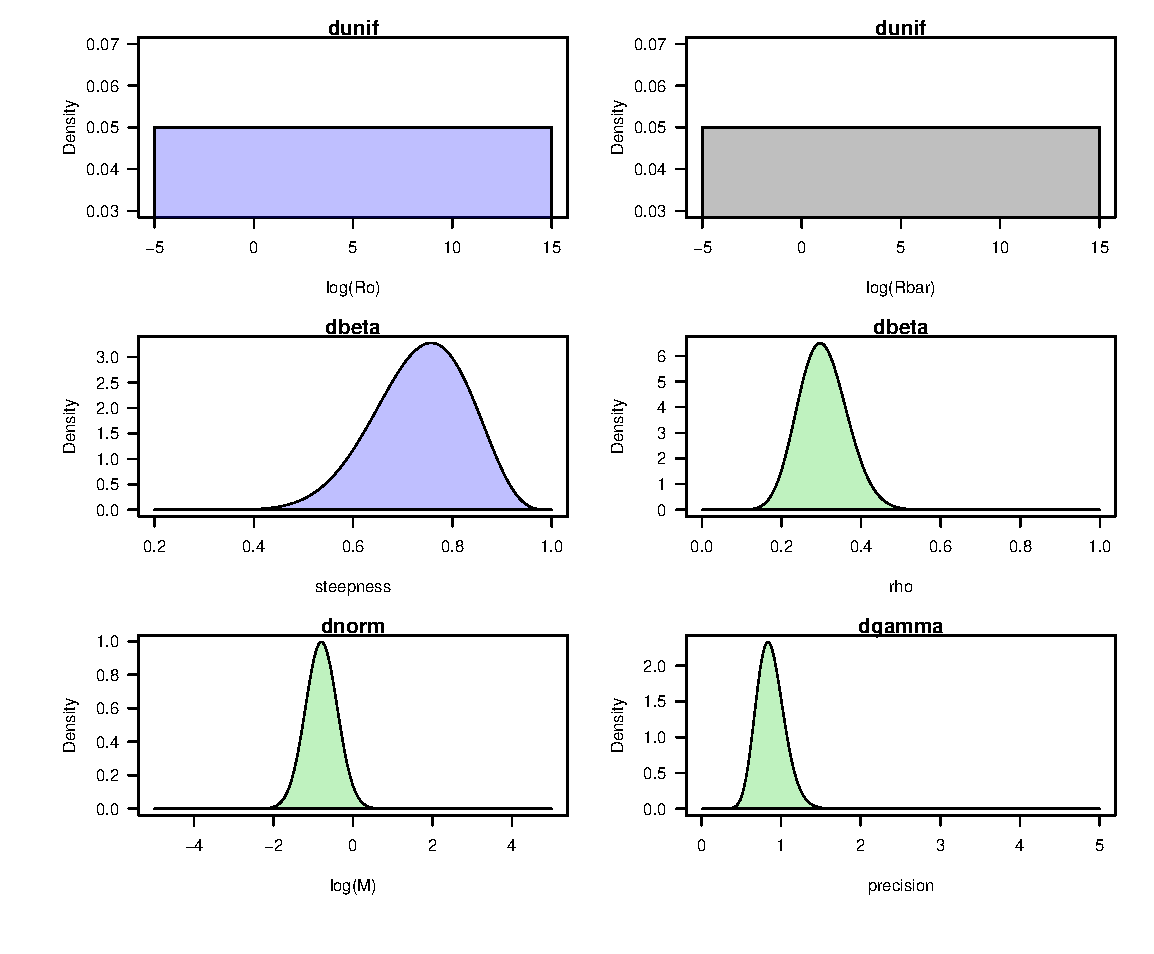
\includegraphics[width=0.7\textwidth]{../FIGS/qPriorFigs/iscam_fig_theta_prior_density.pdf}
		\caption{Prior densities for leading model parameters.}
		\label{fig:priors}
	\end{figure}
\end{frame}

%%% subsubsection model_description (end)

%% subsection analytical_methods (end)

%
\subsection{Simulation testing} % (fold)
\label{sub:simulation_testing}
\begin{frame}[t]\frametitle{Simulation testing}
	Estimation performance with perfect information.\\
	\begin{center}
		\only<1>{
		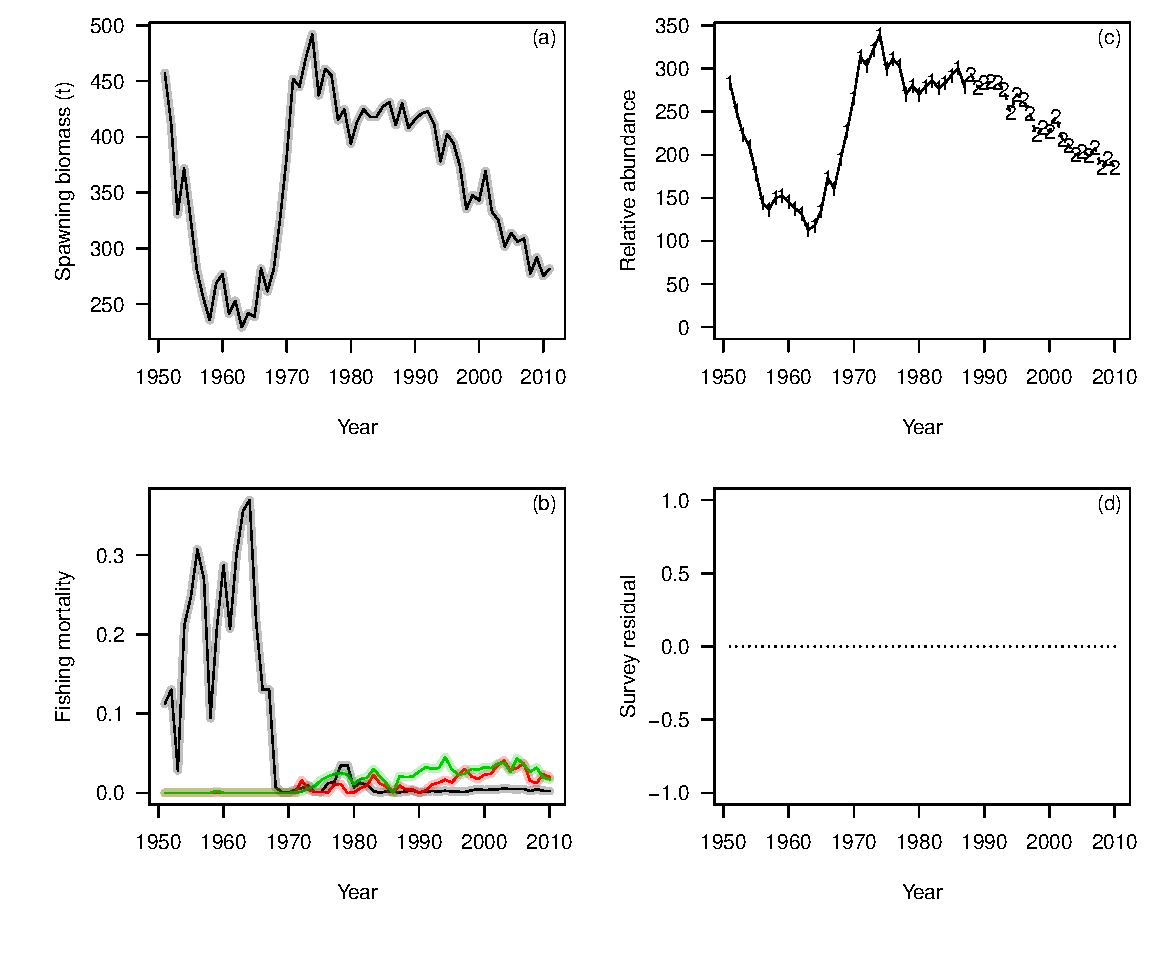
\includegraphics[clip,trim=0 225 260 0,height=0.8\textheight]{../FIGS/simplot}
		}
		\only<2>{
		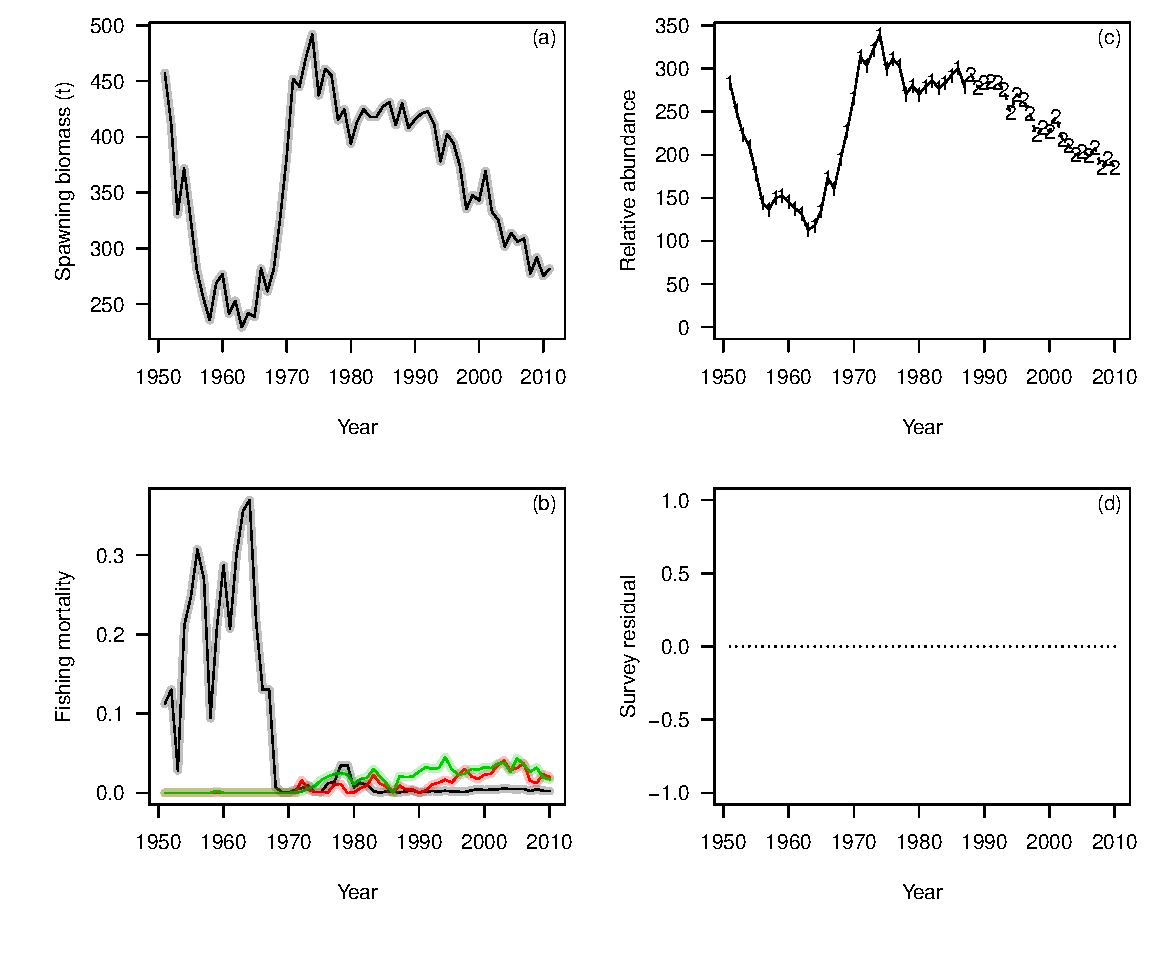
\includegraphics[clip,trim=0 0 260 225,height=0.8\textheight]{../FIGS/simplot}
		}
		\only<3>{
		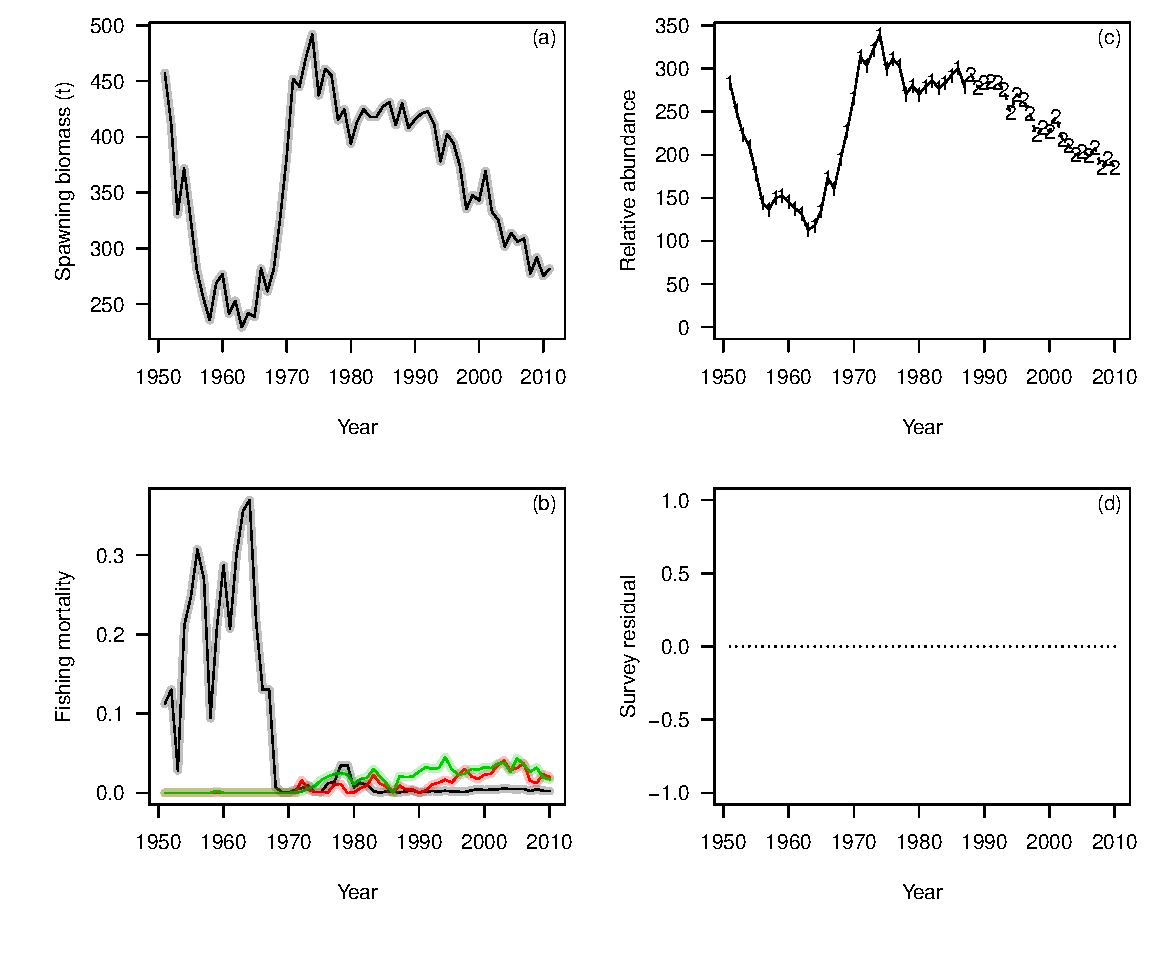
\includegraphics[clip,trim=275 225 0 0,height=0.8\textheight]{../FIGS/simplot}
		}
	\end{center}
	

\end{frame}
%
\begin{frame}[t]\frametitle{Precision \& Bias}
	Bias ratios for key model parameters based on 50 simulated data sets.
	\begin{center}
		\only<1>{
		\includegraphics[clip,trim= 0 250 0 0, width=\textwidth]{../FIGS/SOGparameterBias}
		}
		\only<2>{
		\includegraphics[clip,trim= 0 0 0 220, width=\textwidth]{../FIGS/SOGparameterBias}
		}
	\end{center}
 
\end{frame}
%% subsection simulation_testing (end)

\subsection{SOG Comparison} % (fold)
\label{sub:sog_comparison}
\begin{frame}[t]\frametitle{Strait of Georgia}
	Objective: set up \iscam\ $\sim$ HCAM \& compare.
	\begin{alertblock}
		{Significant differences between \iscam\ \& HCAM}
		\begin{itemize}
			\item<+-> Likelihood for age-comps.
			\item<1-> Pooling of age-proportions less than 2\% into adjacent cohort.
			\item<+-> Conditional MLE for survey $q$.
			\item<+-> Estimation of total variance and variance partitioning parameter ($\vartheta, \rho$).
			\item<+-> Prior for steepness ($h \sim$ Beta in \iscam)
		\end{itemize}
	\end{alertblock}
\end{frame}
%
\begin{frame}[c]\frametitle{SOG Spawning biomass}
	\only<1>{
	\begin{figure}[htbp]
		\centering
			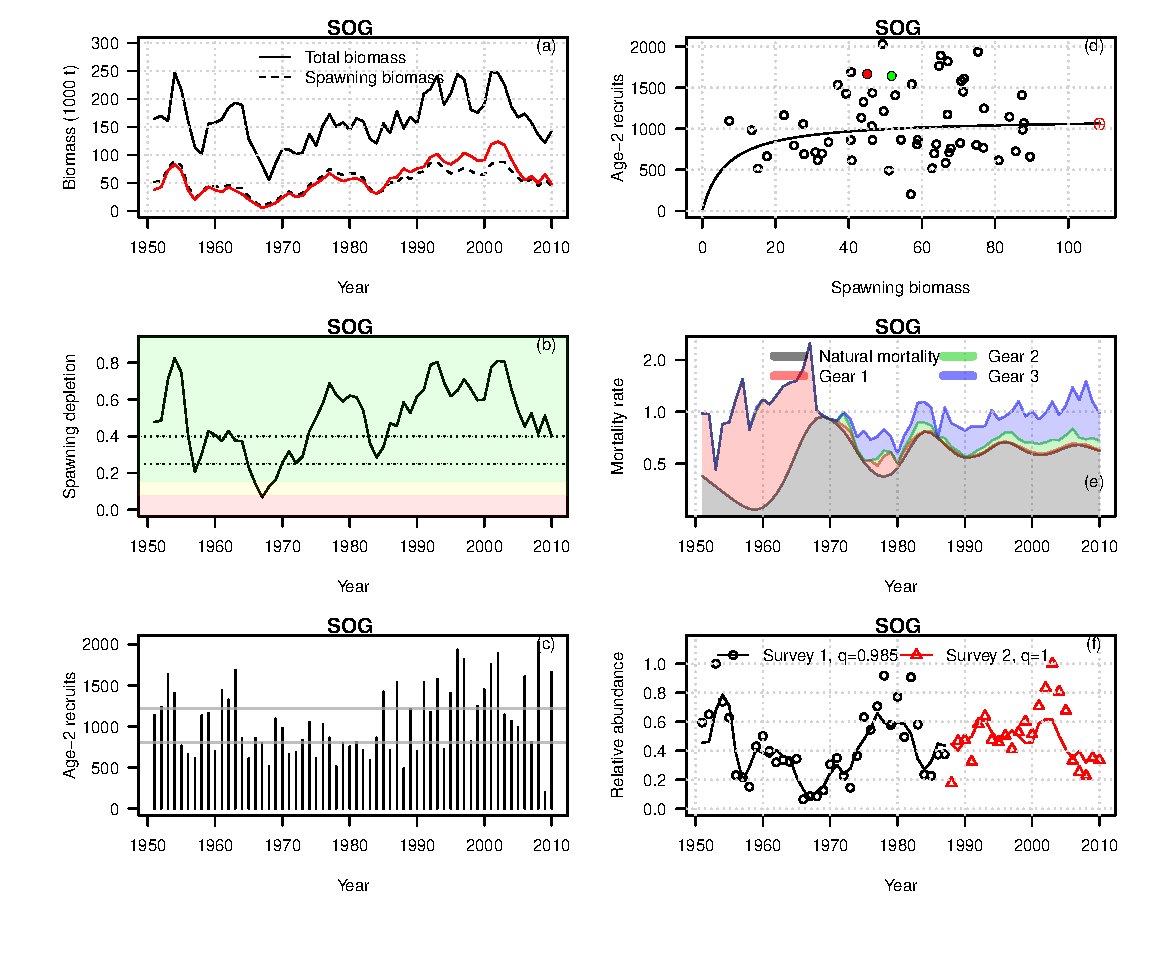
\includegraphics[clip,trim=25 315 270 18,width=\textwidth]
			{../FIGS/iscam_fig_HCAM_SOG_MLE}
		\caption{Total biomass at the start of the year, spawning biomass after fishing. HCAM (2010) spawning biomass shown in red.}
	\end{figure}
	}
	
	\only<2>{
	\begin{figure}[htbp]
		\centering
			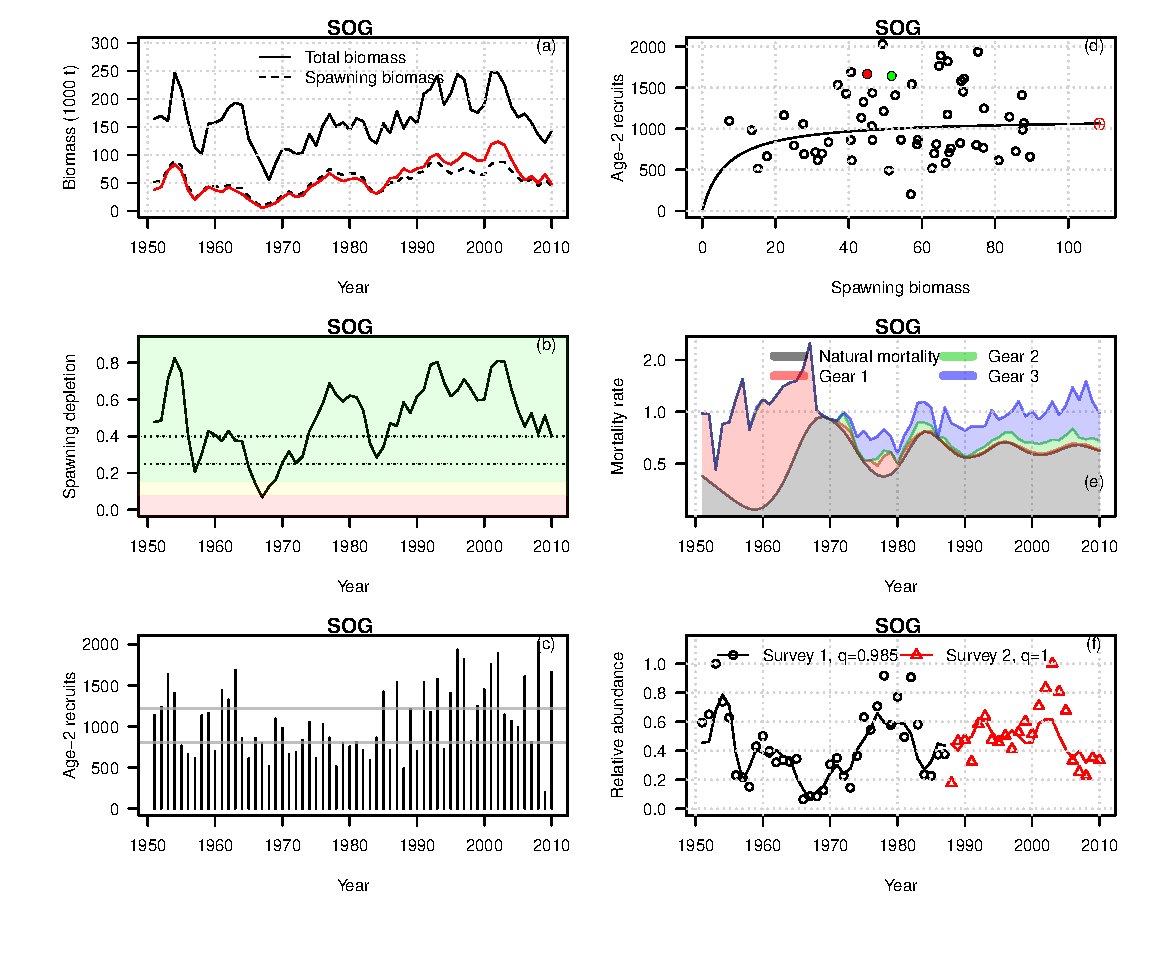
\includegraphics[clip,trim=290 30 0 305,width=\textwidth]
			{../FIGS/iscam_fig_HCAM_SOG_MLE}
		\caption{Observed and predicted spawn survey data for surface (black) and dive (red) surveys.}
	\end{figure}
	}
	
\end{frame}
%% subsection sog_comparison (end)

\subsection{Spawning biomass in major areas} % (fold)
\label{sub:spawning_biomass_in_major_areas}
\begin{frame}[c]
	\only<1>{
	\frametitle{Spawning biomass in HG}
	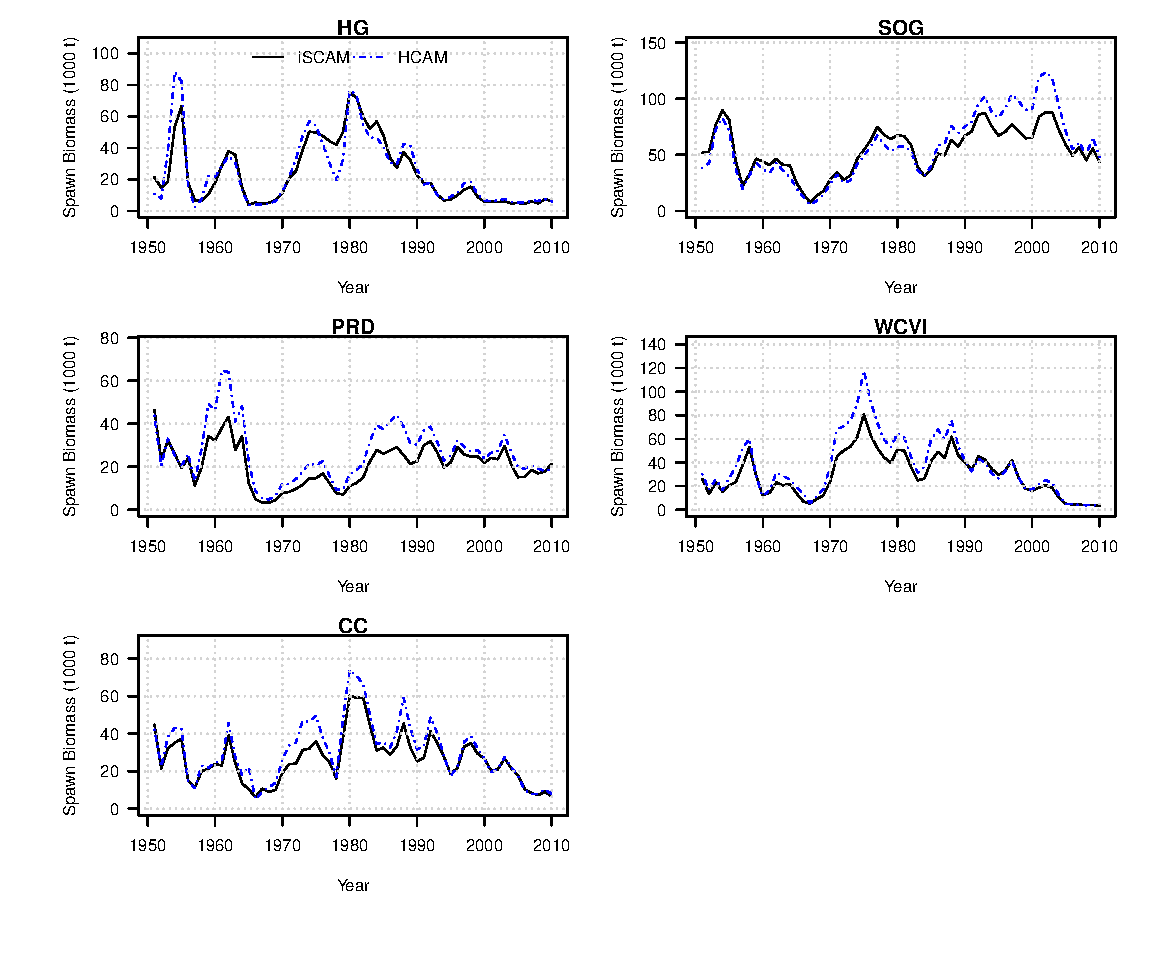
\includegraphics[clip,trim=0cm 10.773cm 9.775cm 0cm]
	{../FIGS/iscam_fig_SBt_iSCAMvsHCAM}
	}
	%
	\only<2>{
	\frametitle{Spawning biomass in PRD}
	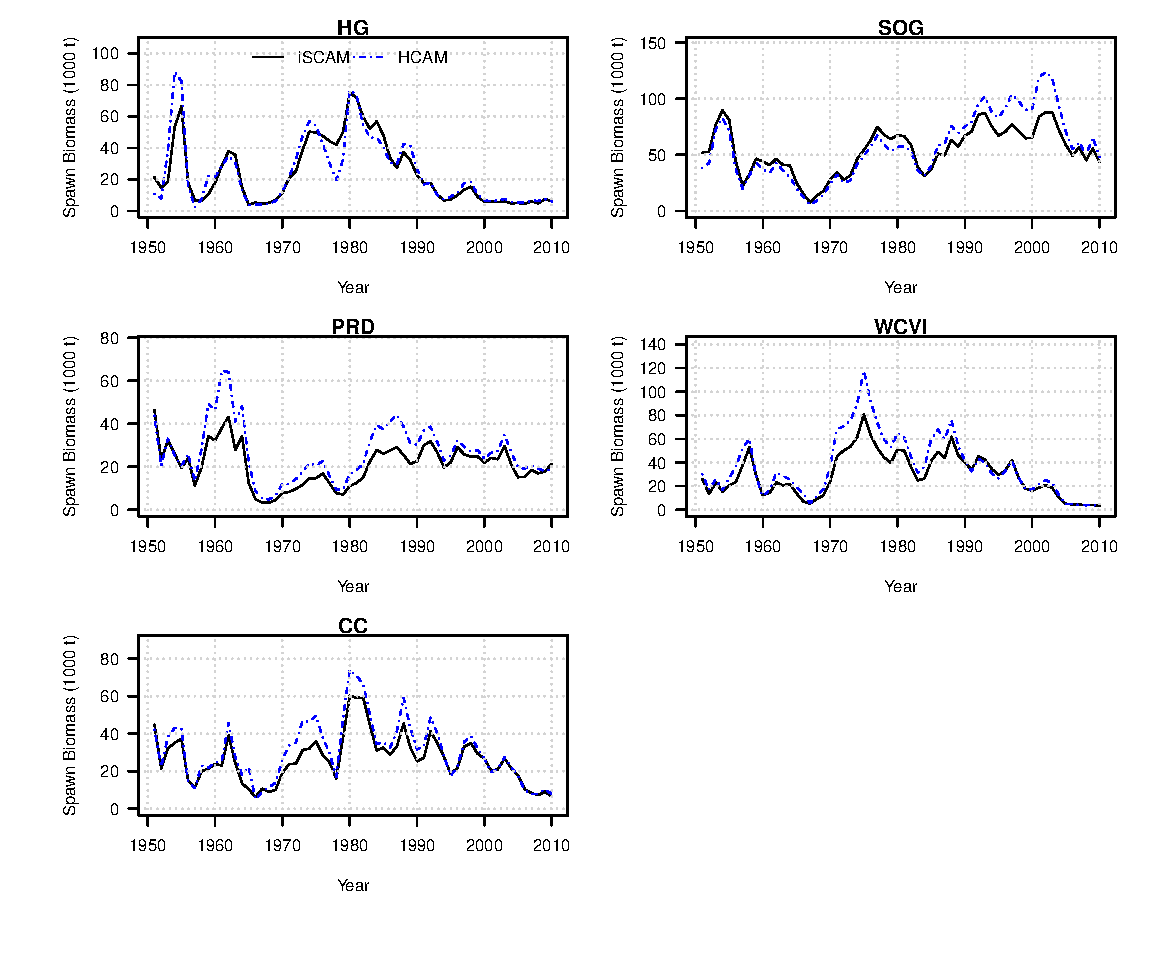
\includegraphics[clip,trim=0cm 5.7cm 9.775cm 5.1cm]
	{../FIGS/iscam_fig_SBt_iSCAMvsHCAM}
	}
	%
	\only<3>{
	\frametitle{Spawning biomass in CC}
	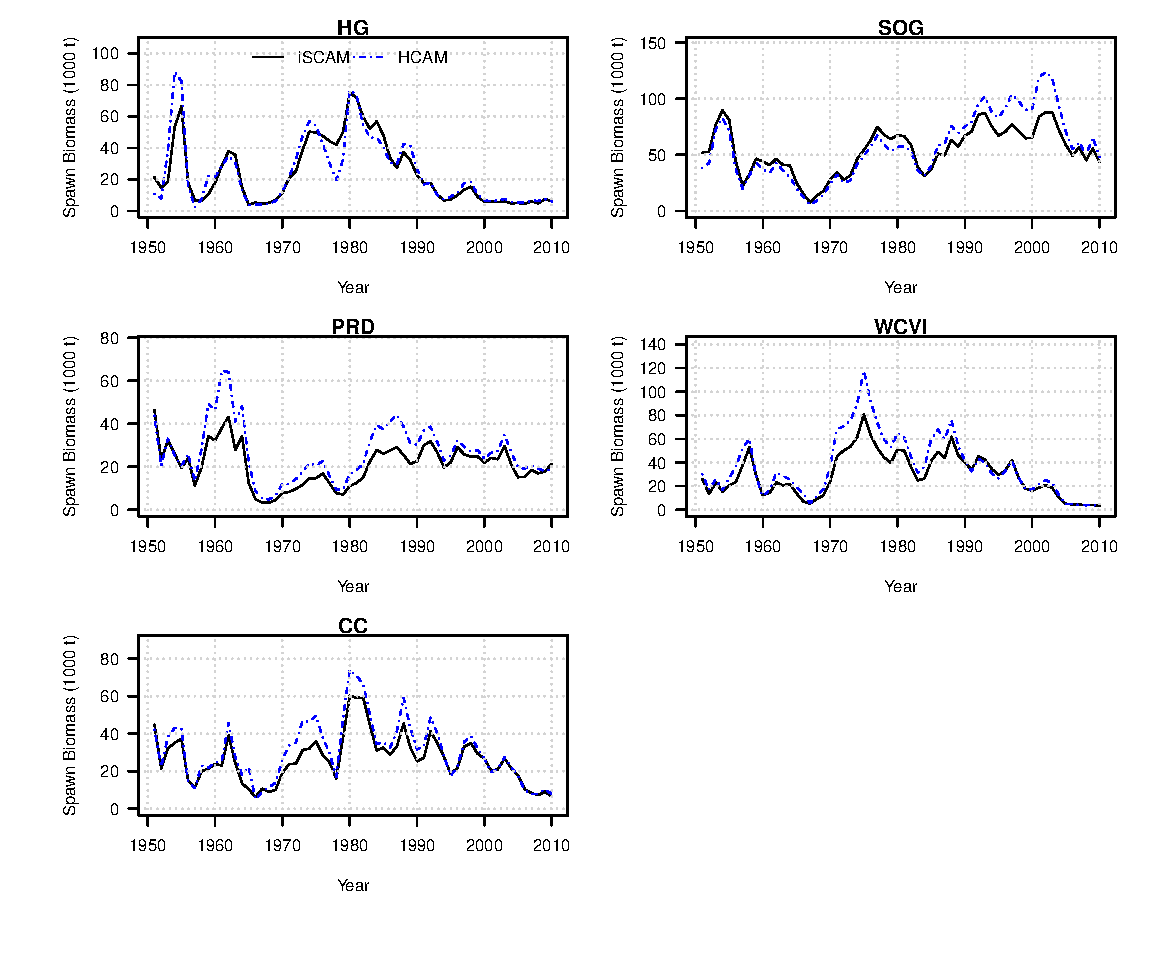
\includegraphics[clip,trim=0cm 0cm 9.775cm 10.4cm]
	{../FIGS/iscam_fig_SBt_iSCAMvsHCAM}
	}
	%
	\only<4>{
	\frametitle{Spawning biomass in SOG}
	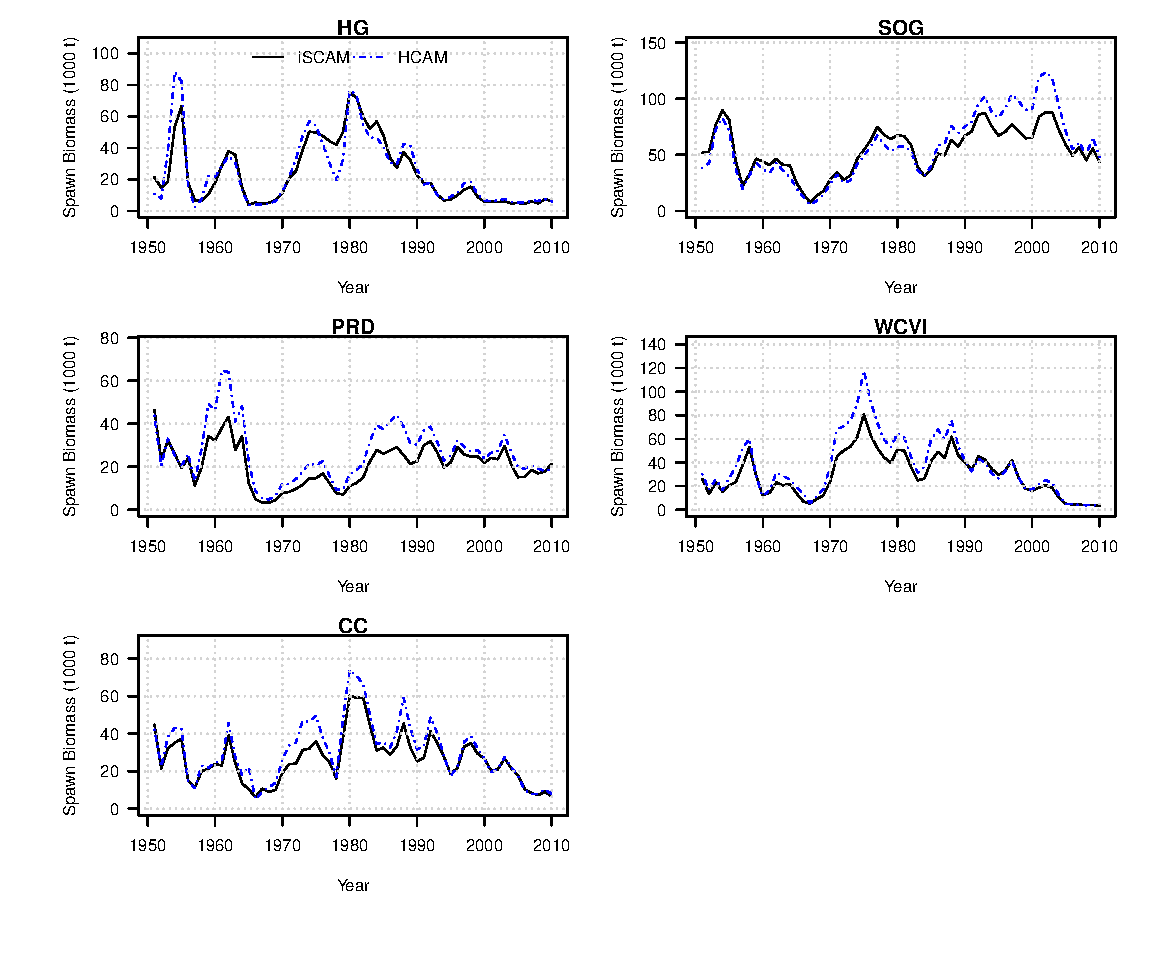
\includegraphics[clip,trim=9.775cm 10.773cm 0cm 0cm]
	{../FIGS/iscam_fig_SBt_iSCAMvsHCAM}
	}
	%
	\only<5>{
	\frametitle{Spawning biomass in WCVI}
	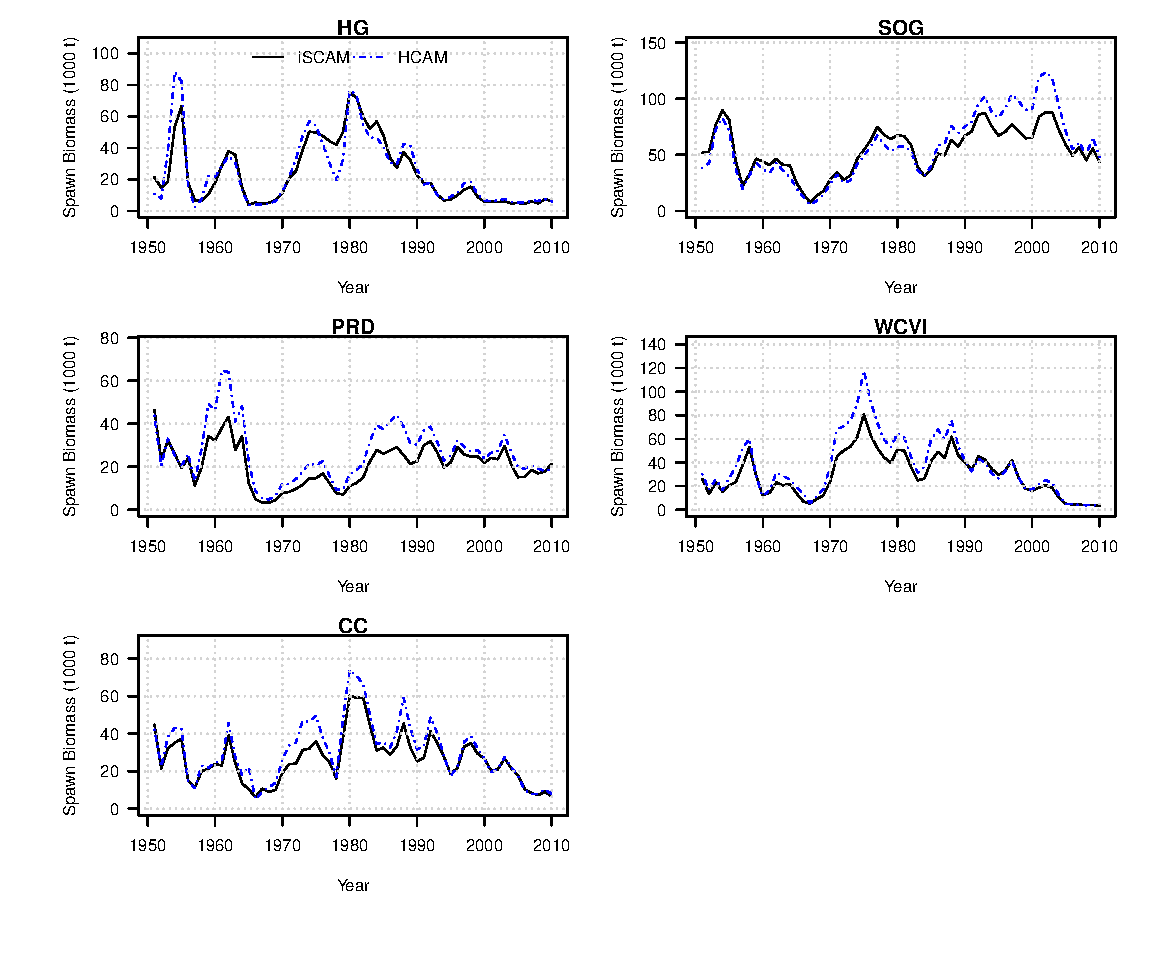
\includegraphics[clip,trim=9.775cm 5.7cm 0cm 5.1cm]
	{../FIGS/iscam_fig_SBt_iSCAMvsHCAM}
	}
\end{frame}
% subsection spawning_biomass_in_major_areas (end)

\subsection{Discussion} % (fold)
\label{sub:discussion}
\begin{frame}[t]\frametitle{Discussion}
	\begin{itemize}
		\item<+-> Slight bias in MSY reference points and steepness; likely due to lack of contrast in simulated data.
		\item<+-> Despite differences between assessment platforms there is a remarkable correspondence in spawning biomass estimates.
		
		\item<+-> Significant differences in:
		\begin{itemize}
			\item weighting of age-composition data,
			\item pooling of age-composition samples ($<$2\%),
			\item conditional MLE for dive survey $q$ with a very informative prior,
			\item prior for steepness.
		\end{itemize}
		\item<+-> MSY based reference points require unbiased estimates of selectivity parameters, and allocation of catch to each gear must be established \textit{a priori}.
	\end{itemize}
\end{frame}
%% subsection discussion (end)
% section part_i (end)
%%_________________________________________________%%






















